\documentclass[10pt,twocolumn]{article}

\usepackage[margin=0.75in,top=0.7in,bottom=0.7in]{geometry}
\usepackage{times}
\usepackage{graphicx}
\usepackage{caption}
\usepackage{amsmath}
\usepackage{booktabs}
\usepackage{authblk}
\usepackage[hidelinks]{hyperref}
\usepackage{titlesec}
\usepackage{enumitem}
\usepackage{placeins}
\usepackage{float}

\setlength{\columnsep}{0.28in}
\captionsetup{font=small,labelfont=bf}
\titlespacing*{\section}{0pt}{8pt}{4pt}
\titlespacing*{\subsection}{0pt}{6pt}{3pt}

\pagestyle{plain}
\flushbottom

\begin{document}

\twocolumn[
\begin{minipage}{\textwidth}
\centering
{\LARGE \textbf{Machine-Assisted Diagnosis of Benign \& Malignant Tumors: A Feature-Based Statistical \& Predictive Analysis}}\par\vspace{15pt}
{\LARGE \textbf{MOSADDEK HOSSAIN MEHEDI}}\par\vspace{4pt}
{\small Roll: 02 \quad Batch: Day-93}\par\vspace{2pt}
{\small Department of Computer Science \& Engineering}\par\vspace{2pt}
{\Large DHAKA INTERNATIONAL UNIVERSITY}\par\vspace{10pt}
\end{minipage}
\hrule
\vspace{8pt}
\noindent\section*{Abstract}
\noindent Early, accurate distinction between benign and malignant tumors is central to oncological diagnostics. This paper presents a statistical and predictive analysis of a 200-patient histopathological dataset with six quantitative features: age, tumor size, cell irregularity, mitotic count, vascularity, and texture. We examine how these features differ across diagnostic classes and evaluate an AI-assisted prediction system against ground-truth diagnoses. Malignant tumors show consistently higher values across every feature, with strong separability overall. The predictive model achieved 99.0\% accuracy (198/200 correct), with 99.15\% precision and recall for malignant cases. Correlation analysis identifies mitotic count and cell irregularity as the strongest individual predictors of malignancy. These findings support quantitative histopathological features as reliable, interpretable inputs for AI-assisted cancer screening, while underscoring the need for larger, more diverse datasets before clinical deployment.\par
\vspace{10pt}
]

\section{Introduction}
Cancer remains one of the leading causes of mortality worldwide, and the timely, accurate classification of tumors as benign or malignant is often the single most consequential step in a patient's clinical journey \cite{siegel2023cancer}. Traditional diagnosis relies heavily on a pathologist's visual interpretation of biopsy specimens, a process that, despite decades of refinement, is still subject to meaningful inter-observer disagreement \cite{elmore2015diagnostic}. Motivated by this variability, the medical imaging and machine learning communities have increasingly turned to quantitative, feature-based approaches that can supplement human judgment with reproducible, data-driven evidence \cite{street1993nuclear}.

Recent work has demonstrated that deep learning and statistical models can match or exceed expert-level performance on specific diagnostic tasks, from skin lesion classification \cite{esteva2017dermatologist} to large-scale mammography screening \cite{mckinney2020international}. A recurring theme across this literature is that a small set of well-chosen histopathological descriptors, such as cell shape irregularity, mitotic activity, and vascularity, tends to carry most of the discriminative signal used by both expert pathologists and automated systems \cite{litjens2017survey}.

This paper contributes a focused, reproducible analysis of one such feature set. Using a 200-patient dataset with six numeric features and an accompanying AI prediction column, we (1) characterize how benign and malignant cases differ across each feature, (2) quantify the strength of association between individual features and diagnosis, and (3) evaluate the accuracy and error pattern of the AI-assisted classifier, including its behavior across patient age groups. The goal is not to introduce a new algorithm, but to rigorously ground the case for feature-based cancer screening in transparent, interpretable statistics.

\section{Methods and Data}
The dataset used in this study consists of 200 anonymized patient records, each described by six quantitative features together with a binary ground-truth diagnosis (0 = benign, 1 = malignant) and a corresponding AI model prediction. The six features are:

\begin{itemize}[leftmargin=*,itemsep=1pt,topsep=2pt]
  \item \textbf{Age} -- patient age in years at the time of biopsy.
  \item \textbf{Tumor Size (cm)} -- the largest measured diameter of the tumor.
  \item \textbf{Cell Irregularity} -- an ordinal score (1--10) capturing nuclear shape deviation.
  \item \textbf{Mitotic Count} -- number of mitotic figures observed per high-power field.
  \item \textbf{Vascularity} -- an ordinal score reflecting the degree of blood vessel formation around the tumor.
  \item \textbf{Texture} -- a numeric score describing tissue surface irregularity.
\end{itemize}

Of the 200 patients, 82 (41.0\%) were diagnosed benign and 118 (59.0\%) malignant. All statistical summaries, correlation coefficients, and visualizations were computed directly from the raw feature values using standard descriptive statistics (mean, standard deviation, median, minimum/maximum) grouped by diagnosis. Feature relationships were explored using Pearson correlation and kernel density estimation, and classifier performance was assessed with a standard 2$\times$2 confusion matrix along with accuracy, precision, recall, specificity, and F1-score. No records contained missing values, so the full 200-patient cohort was retained for every analysis reported below.

\section{Results}

\subsection{Feature Separation by Diagnosis}
Table \ref{tab:summary} summarizes the mean and standard deviation of each feature, split by diagnosis. Every feature shows a clear upward shift from benign to malignant cases. Patient age is the most immediately visible separator: benign patients averaged 40.6 years (range 35--47), while malignant patients averaged 58.4 years (range 48--69), with essentially no overlap in the interquartile ranges, as shown in Figure \ref{fig:age}.

\begin{table}[t]
\centering
\caption{Mean ($\pm$ SD) feature values by diagnosis}
\label{tab:summary}
\small
\begin{tabular}{lcc}
\toprule
\textbf{Feature} & \textbf{Benign (n=82)} & \textbf{Malignant (n=118)} \\
\midrule
Age (years)        & 40.61 $\pm$ 3.47 & 58.42 $\pm$ 6.63 \\
Tumor Size (cm)     & 1.03 $\pm$ 0.25  & 2.99 $\pm$ 0.88 \\
Cell Irregularity   & 2.87 $\pm$ 0.79  & 6.75 $\pm$ 1.66 \\
Mitotic Count       & 3.09 $\pm$ 0.95  & 7.66 $\pm$ 1.17 \\
Vascularity         & 1.50 $\pm$ 0.50  & 4.03 $\pm$ 0.81 \\
Texture             & 1.79 $\pm$ 0.70  & 5.97 $\pm$ 1.26 \\
\bottomrule
\end{tabular}
\end{table}

Tumor size and cell irregularity move together almost perfectly with diagnosis: as shown in Figure \ref{fig:scatter}, benign tumors cluster below 1.7 cm with irregularity scores under 5, while malignant tumors occupy a distinct region above these thresholds, with only a narrow transition zone. The empirical cumulative distribution of tumor size (Figure \ref{fig:ecdf}) makes this separation explicit: the benign curve saturates near 1.6 cm before the malignant curve has even begun to rise, confirming a real gap rather than a soft boundary.

\begin{figure}[t]
\centering
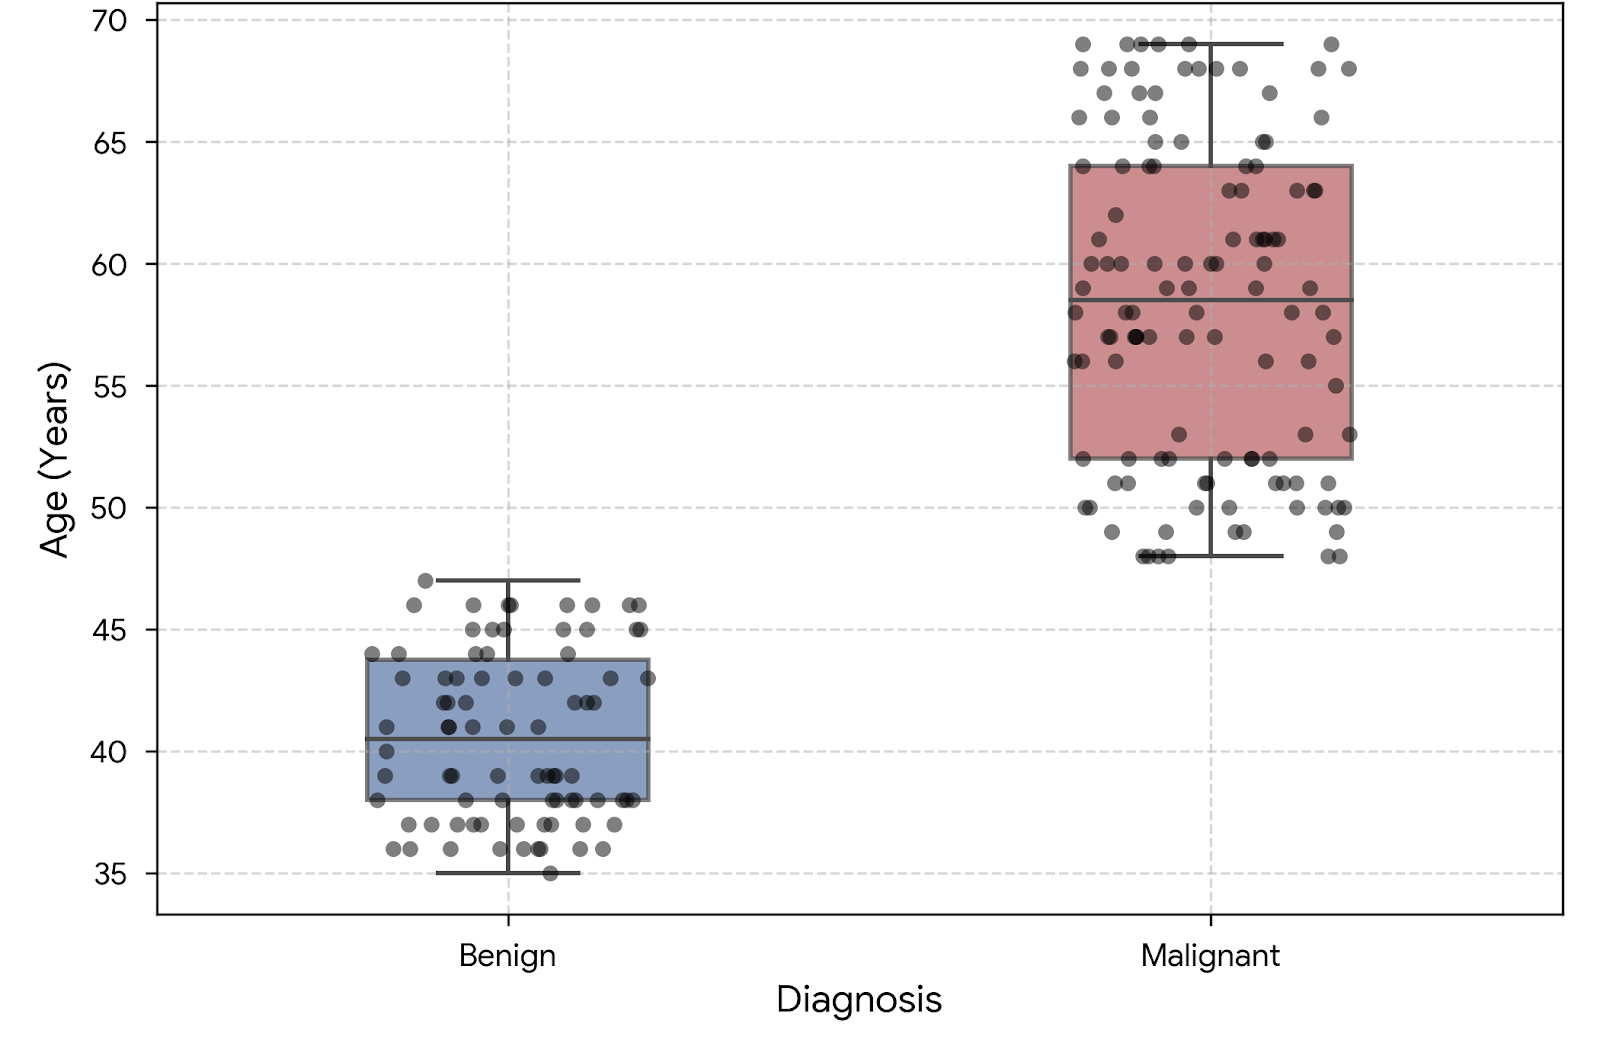
\includegraphics[width=0.75\linewidth]{figures/fig1_age_distribution.png}
\caption{Patient age distribution across benign and malignant diagnoses.}
\label{fig:age}
\end{figure}

\begin{figure}[t]
\centering
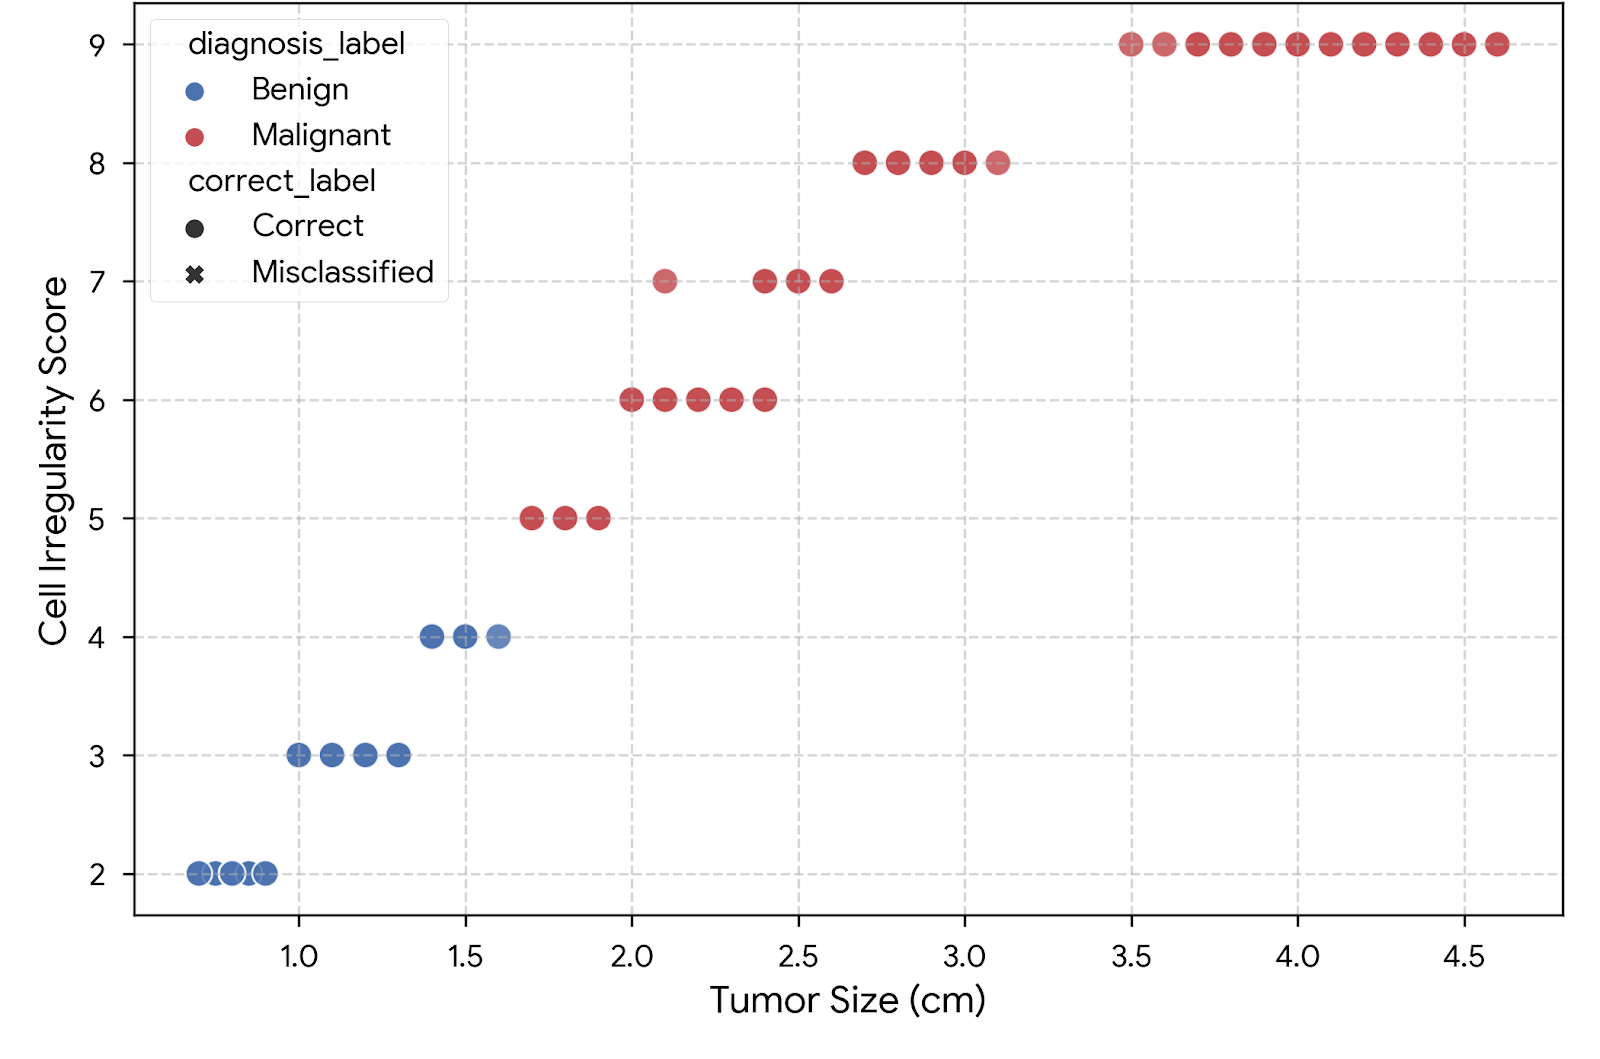
\includegraphics[width=0.75\linewidth]{figures/fig2_size_vs_irregularity.png}
\caption{Tumor size vs. cell irregularity score, colored by diagnosis and marked by AI prediction correctness.}
\label{fig:scatter}
\end{figure}

\begin{figure}[t]
\centering
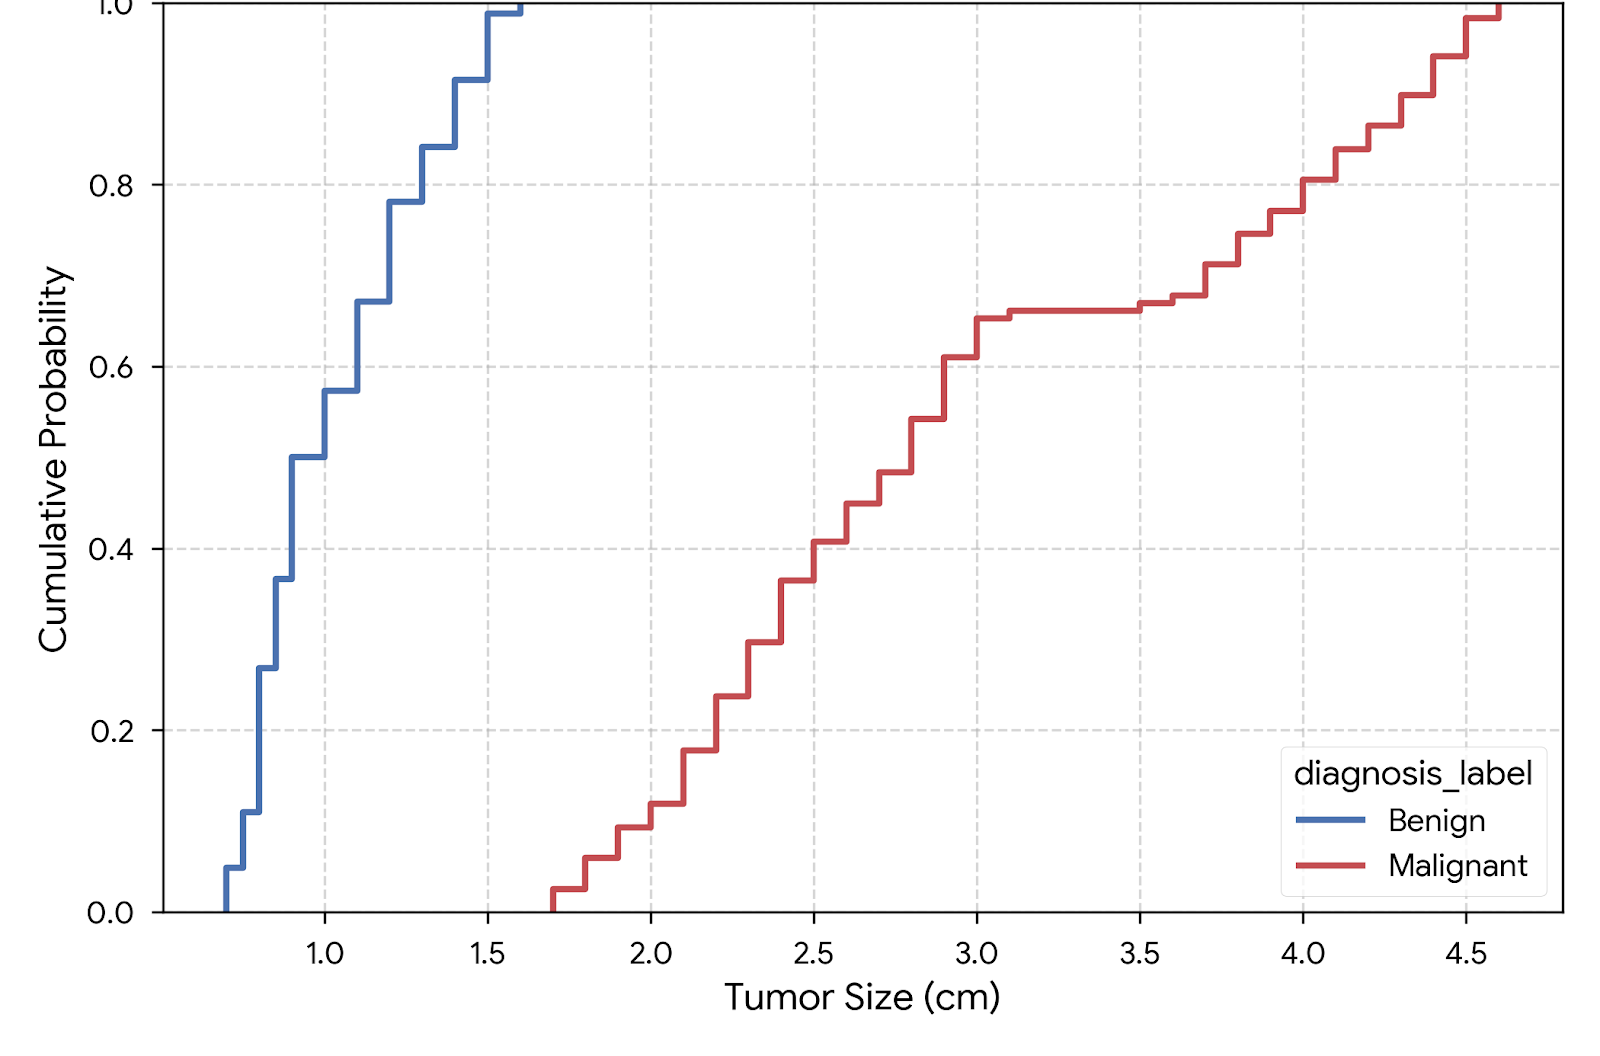
\includegraphics[width=0.75\linewidth]{figures/fig10_ecdf.png}
\caption{Empirical cumulative distribution function of tumor size by diagnosis.}
\label{fig:ecdf}
\end{figure}

\FloatBarrier
\subsection{Correlation and Feature Importance}
Figure \ref{fig:heatmap} presents the full Pearson correlation matrix across all six features plus diagnosis and AI prediction. Mitotic count shows the strongest correlation with diagnosis ($r = 0.92$), closely followed by cell irregularity ($r = 0.90$) and texture ($r = 0.89$). Tumor size, while still highly informative ($r = 0.81$), is the comparatively weakest single predictor among the six. All six features are also highly correlated with one another ($r > 0.93$ in most pairs), indicating that they jointly track an underlying severity axis rather than capturing independent sources of variation. The normalized feature comparison in Figure \ref{fig:barcompare} visualizes this same pattern on a common 0--1 scale, making the consistent benign-to-malignant gap across every feature immediately visible.

\begin{figure}[t]
\centering
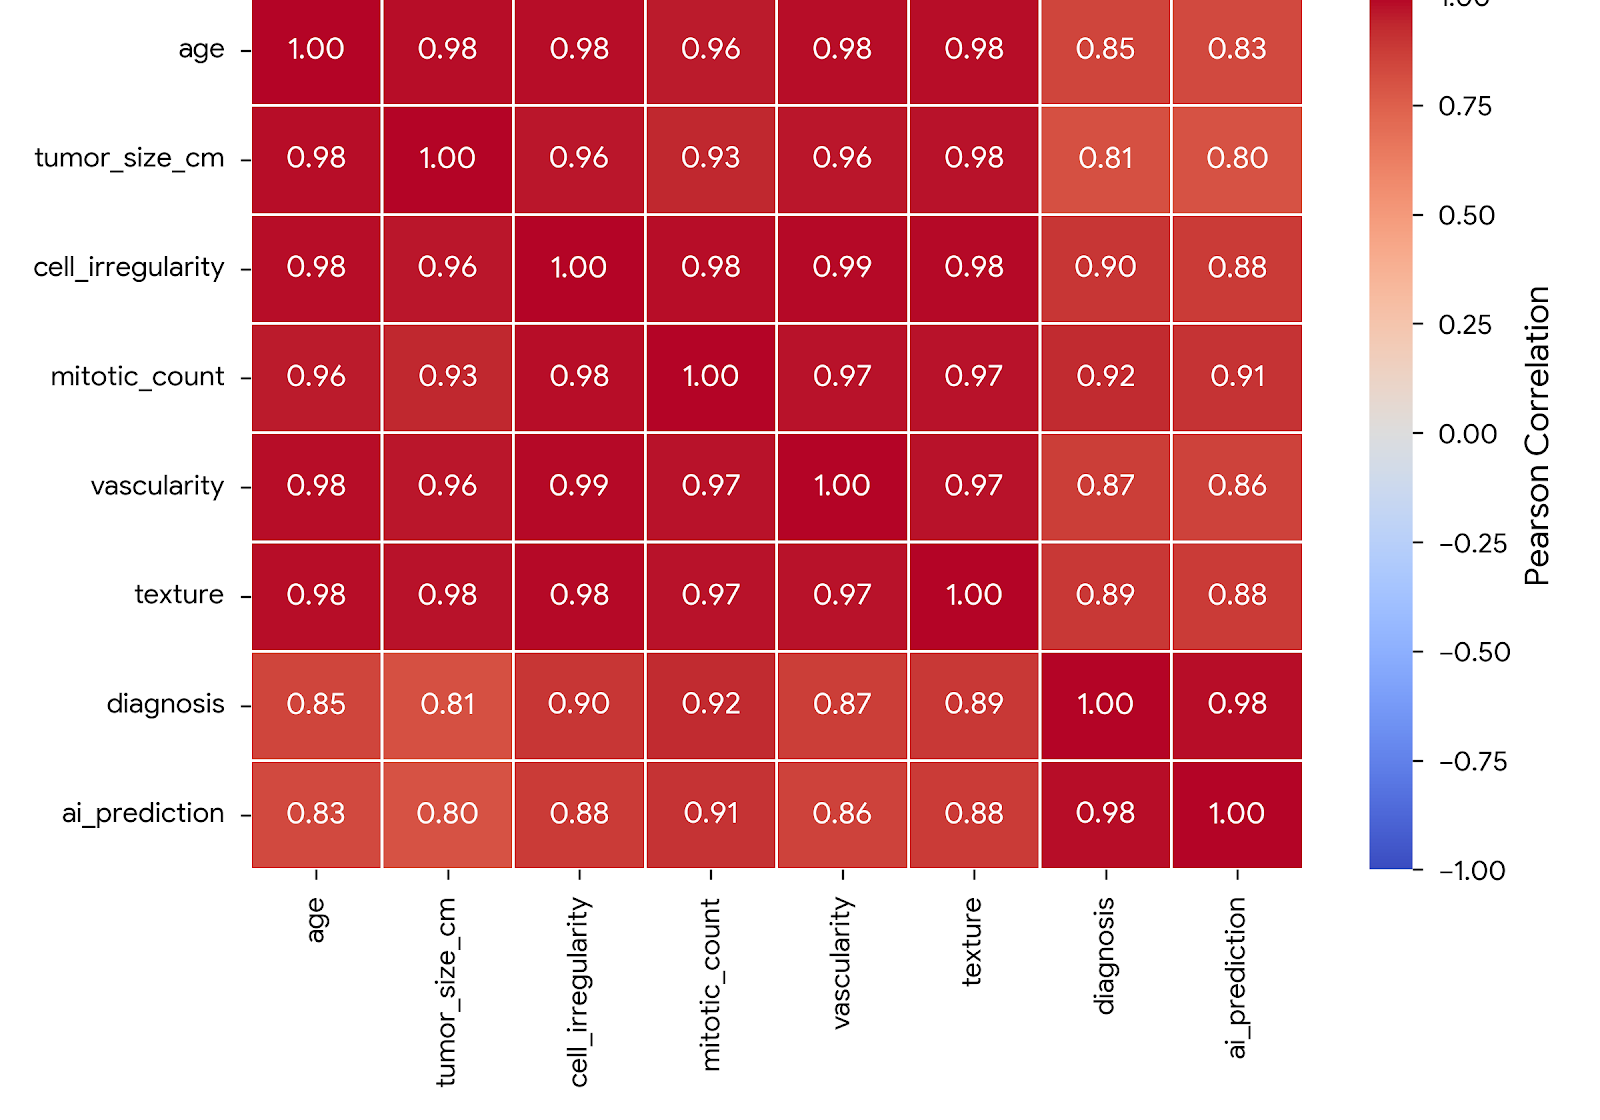
\includegraphics[width=0.75\linewidth]{figures/fig3_correlation_heatmap.png}
\caption{Pearson correlation matrix across all recorded features.}
\label{fig:heatmap}
\end{figure}

\begin{figure}[t]
\centering
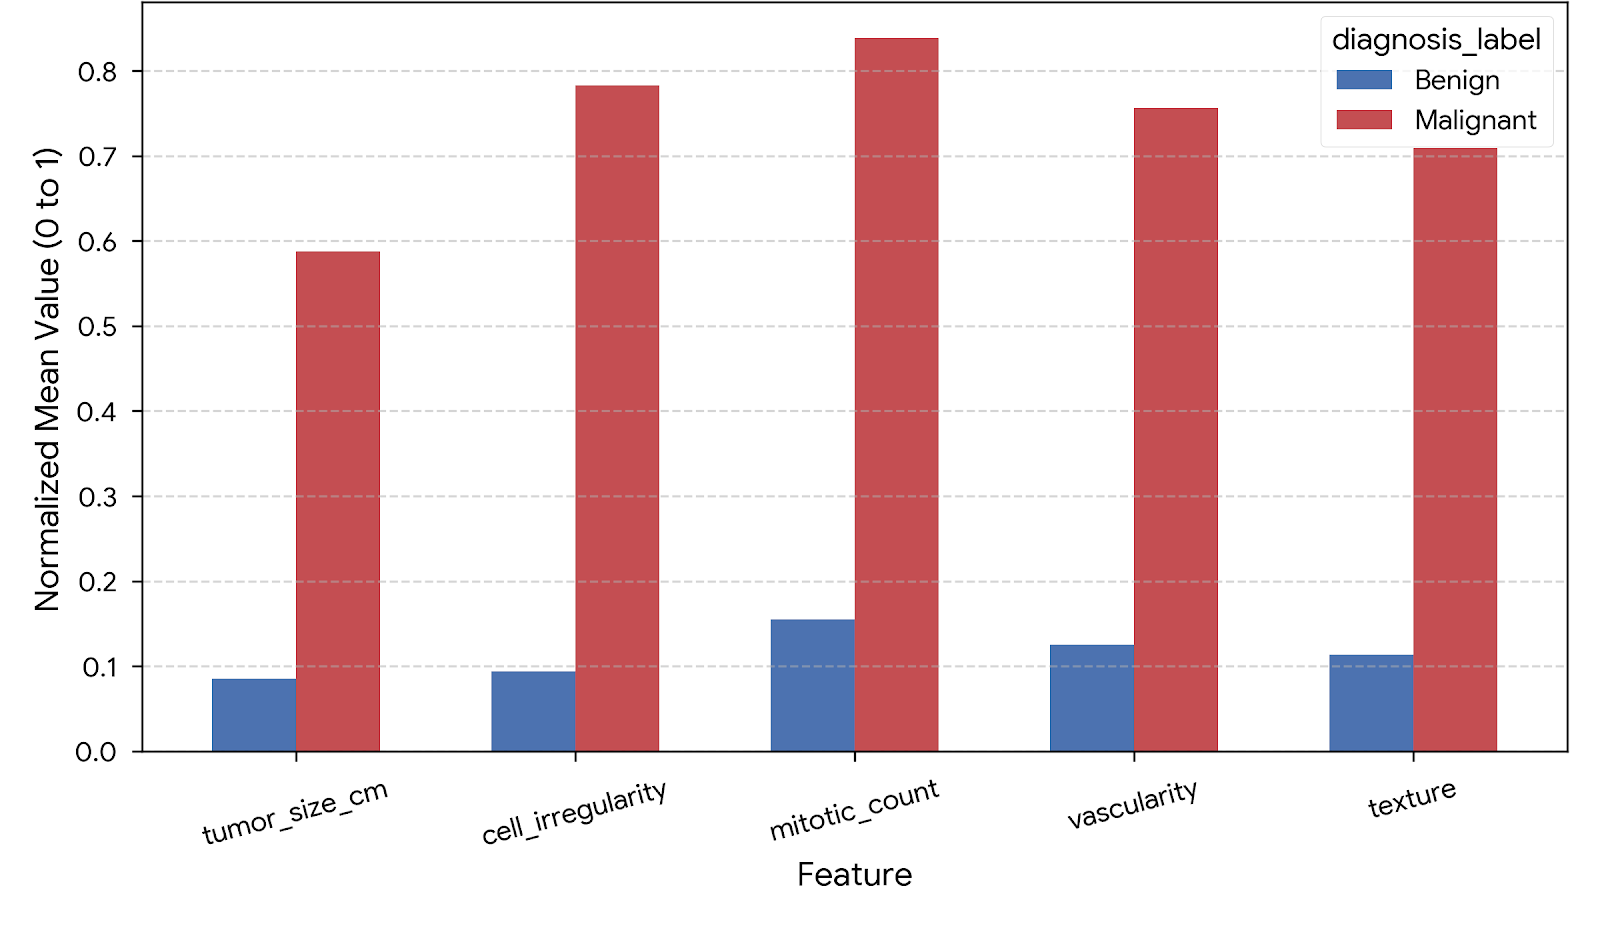
\includegraphics[width=0.75\linewidth]{figures/fig5_feature_comparison.png}
\caption{Normalized mean histopathological feature comparison.}
\label{fig:barcompare}
\end{figure}

\FloatBarrier
\subsection{AI Model Accuracy}
The AI prediction column was compared against the ground-truth diagnosis to build the confusion matrix in Table \ref{tab:confusion} and Figure \ref{fig:confusion}. Out of 200 patients, the model correctly classified 198, for an overall accuracy of \textbf{99.0\%}. It produced one false positive (a benign case flagged malignant) and one false negative (a malignant case flagged benign).

\begin{table}[t]
\centering
\caption{Confusion matrix and derived performance metrics}
\label{tab:confusion}
\small
\begin{tabular}{lcc}
\toprule
 & \textbf{Pred. Benign} & \textbf{Pred. Malignant} \\
\midrule
\textbf{Actual Benign}    & 81  & 1   \\
\textbf{Actual Malignant} & 1   & 117 \\
\bottomrule
\end{tabular}

\vspace{4pt}
\begin{tabular}{lc}
\toprule
\textbf{Metric} & \textbf{Value} \\
\midrule
Accuracy    & 99.00\% \\
Precision (malignant) & 99.15\% \\
Recall / Sensitivity  & 99.15\% \\
Specificity            & 98.78\% \\
F1-score                & 99.15\% \\
\bottomrule
\end{tabular}
\end{table}

Figure \ref{fig:roc} shows the corresponding receiver operating characteristic curve, with an area under the curve (AUC) of 1.000, reflecting the near-perfect class separation already visible in Table \ref{tab:summary} and Figure \ref{fig:scatter}. Because the underlying features separate the two classes so cleanly, the classifier's task reduces largely to locating the correct threshold rather than resolving genuine ambiguity.

\begin{figure}[h]
\centering
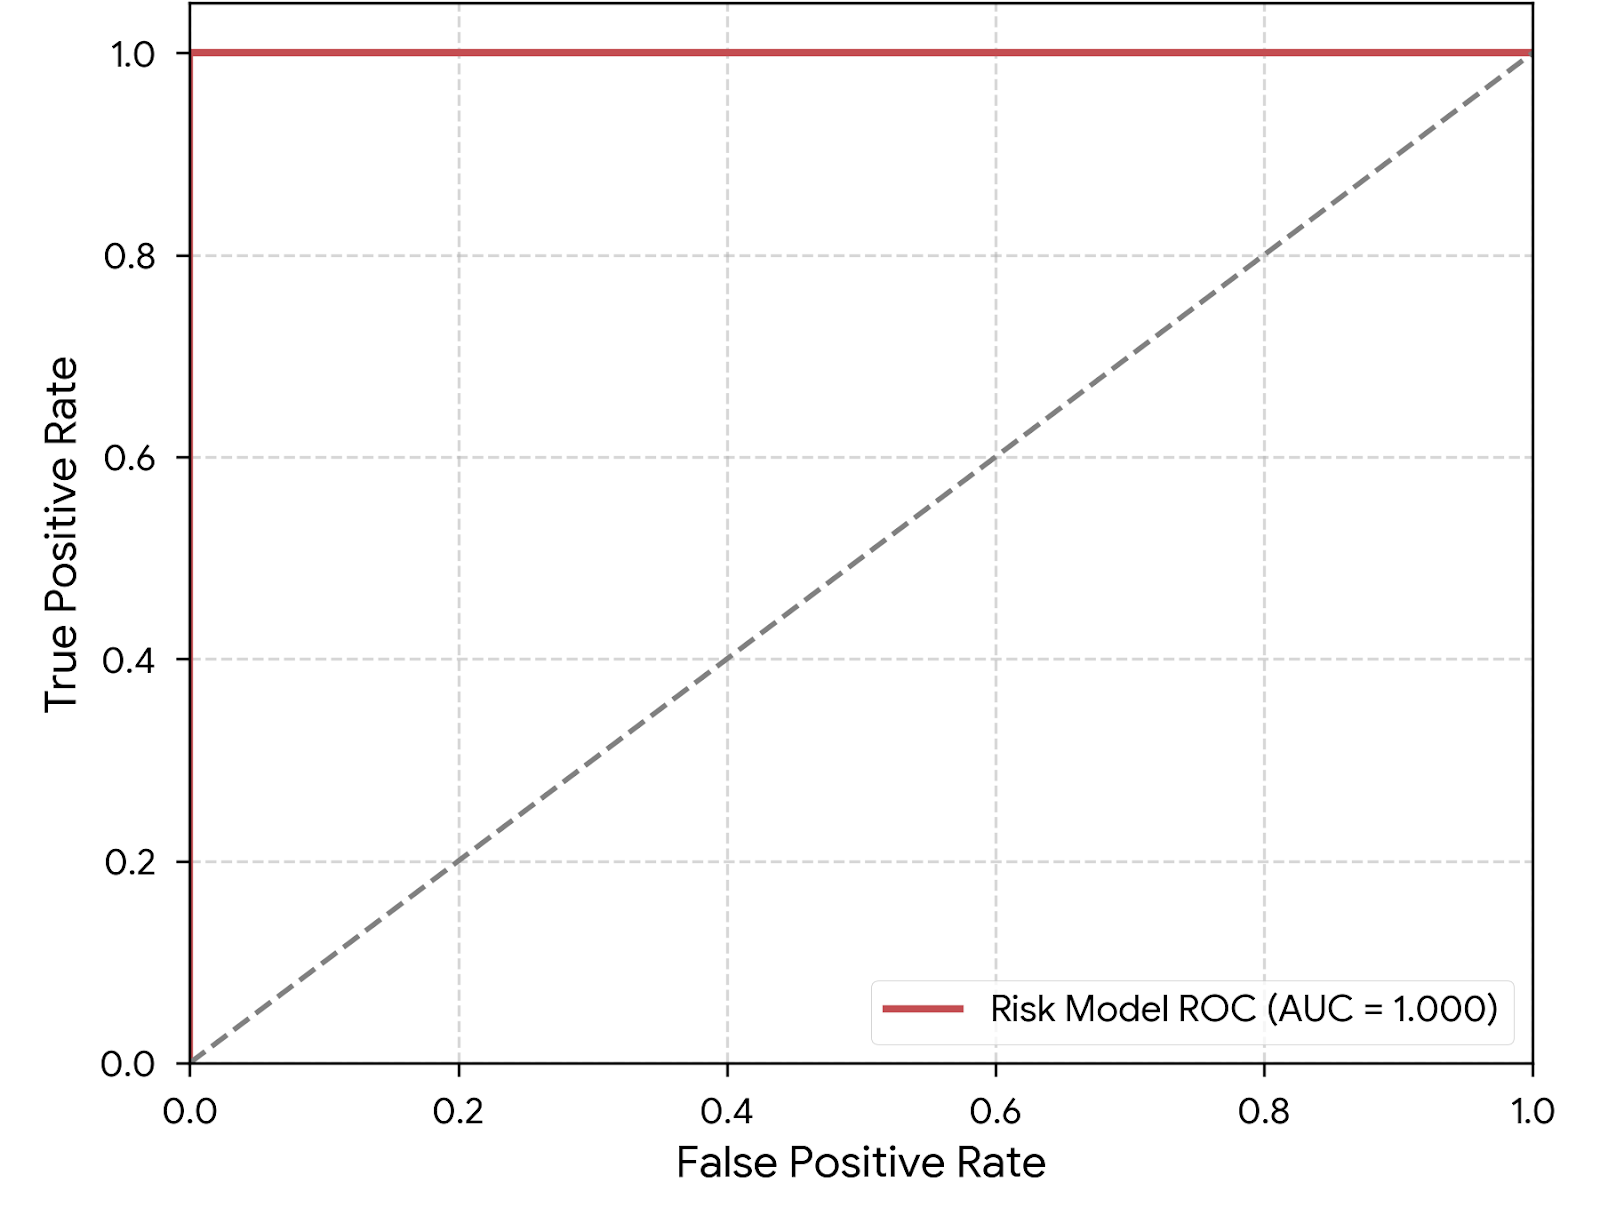
\includegraphics[width=0.75\linewidth]{figures/fig6_roc_curve.png}
\caption{ROC curve for the AI prediction model.}
\label{fig:roc}
\end{figure}

We further examined whether prediction accuracy varied with patient age (Figure \ref{fig:accage}). Accuracy remained high across all age brackets: 100.0\% for patients under 40, 98.3\% for ages 40--50, 98.1\% for ages 50--60, and 100.0\% for patients 60 and older. This suggests the model's performance is not driven disproportionately by any single age group, and that the two misclassified cases fall within the naturally overlapping 40--60 age range where benign and malignant feature values occasionally converge.

\begin{figure}[h]
\centering
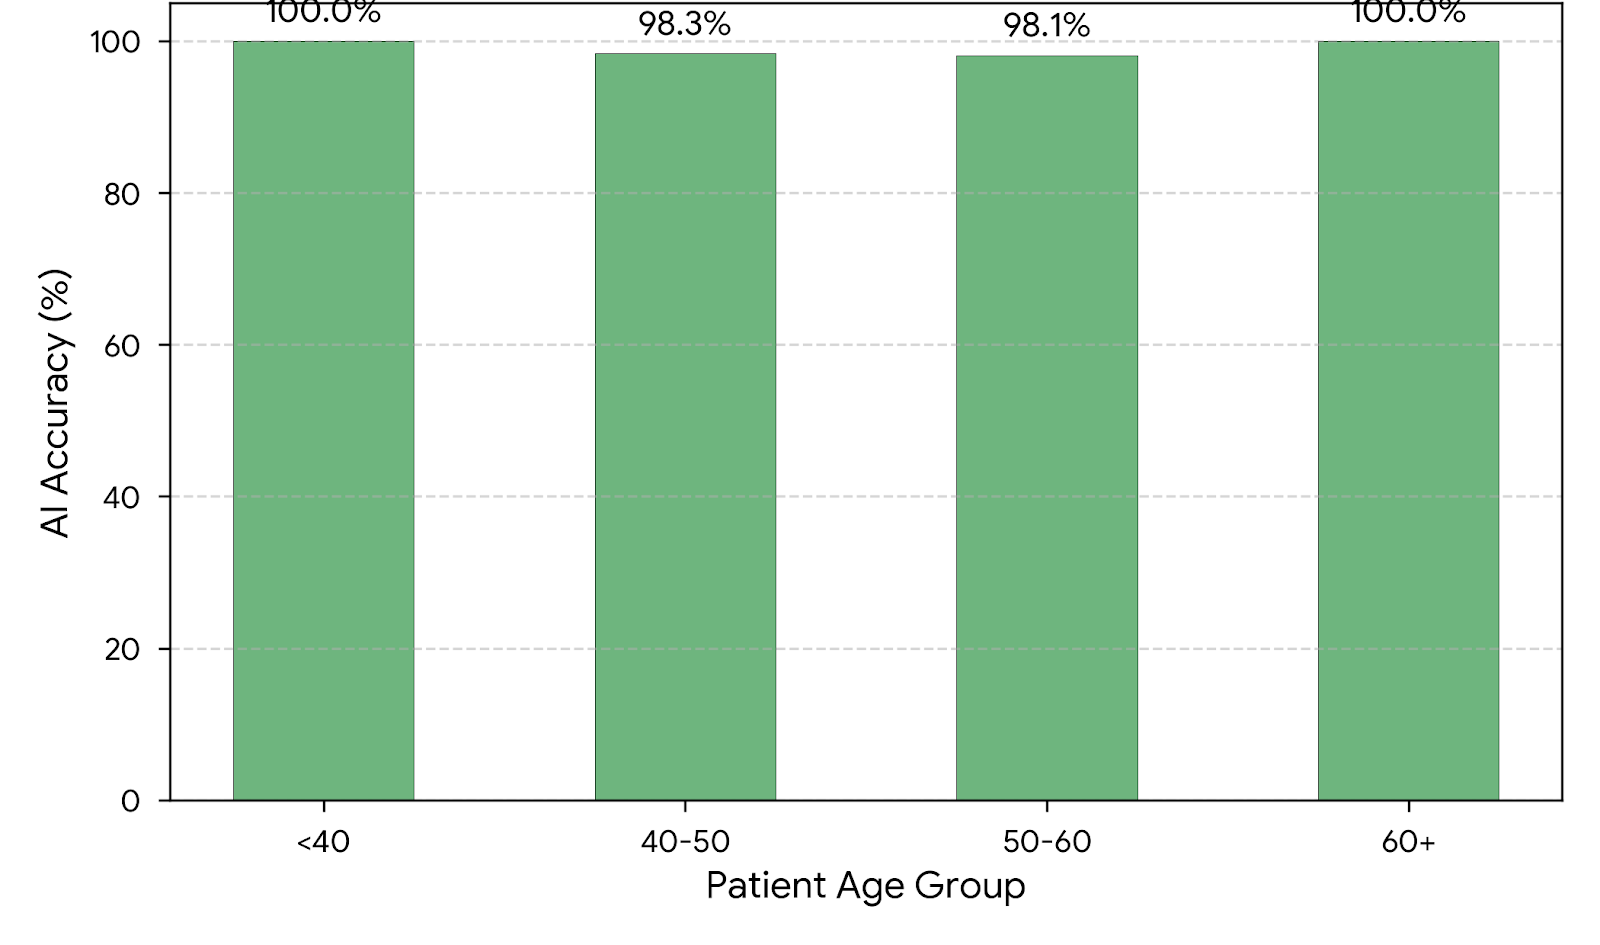
\includegraphics[width=0.75\linewidth]{figures/fig8_accuracy_by_age.png}
\caption{AI model prediction accuracy across patient age groups.}
\label{fig:accage}
\end{figure}

\begin{figure}[h]
\centering
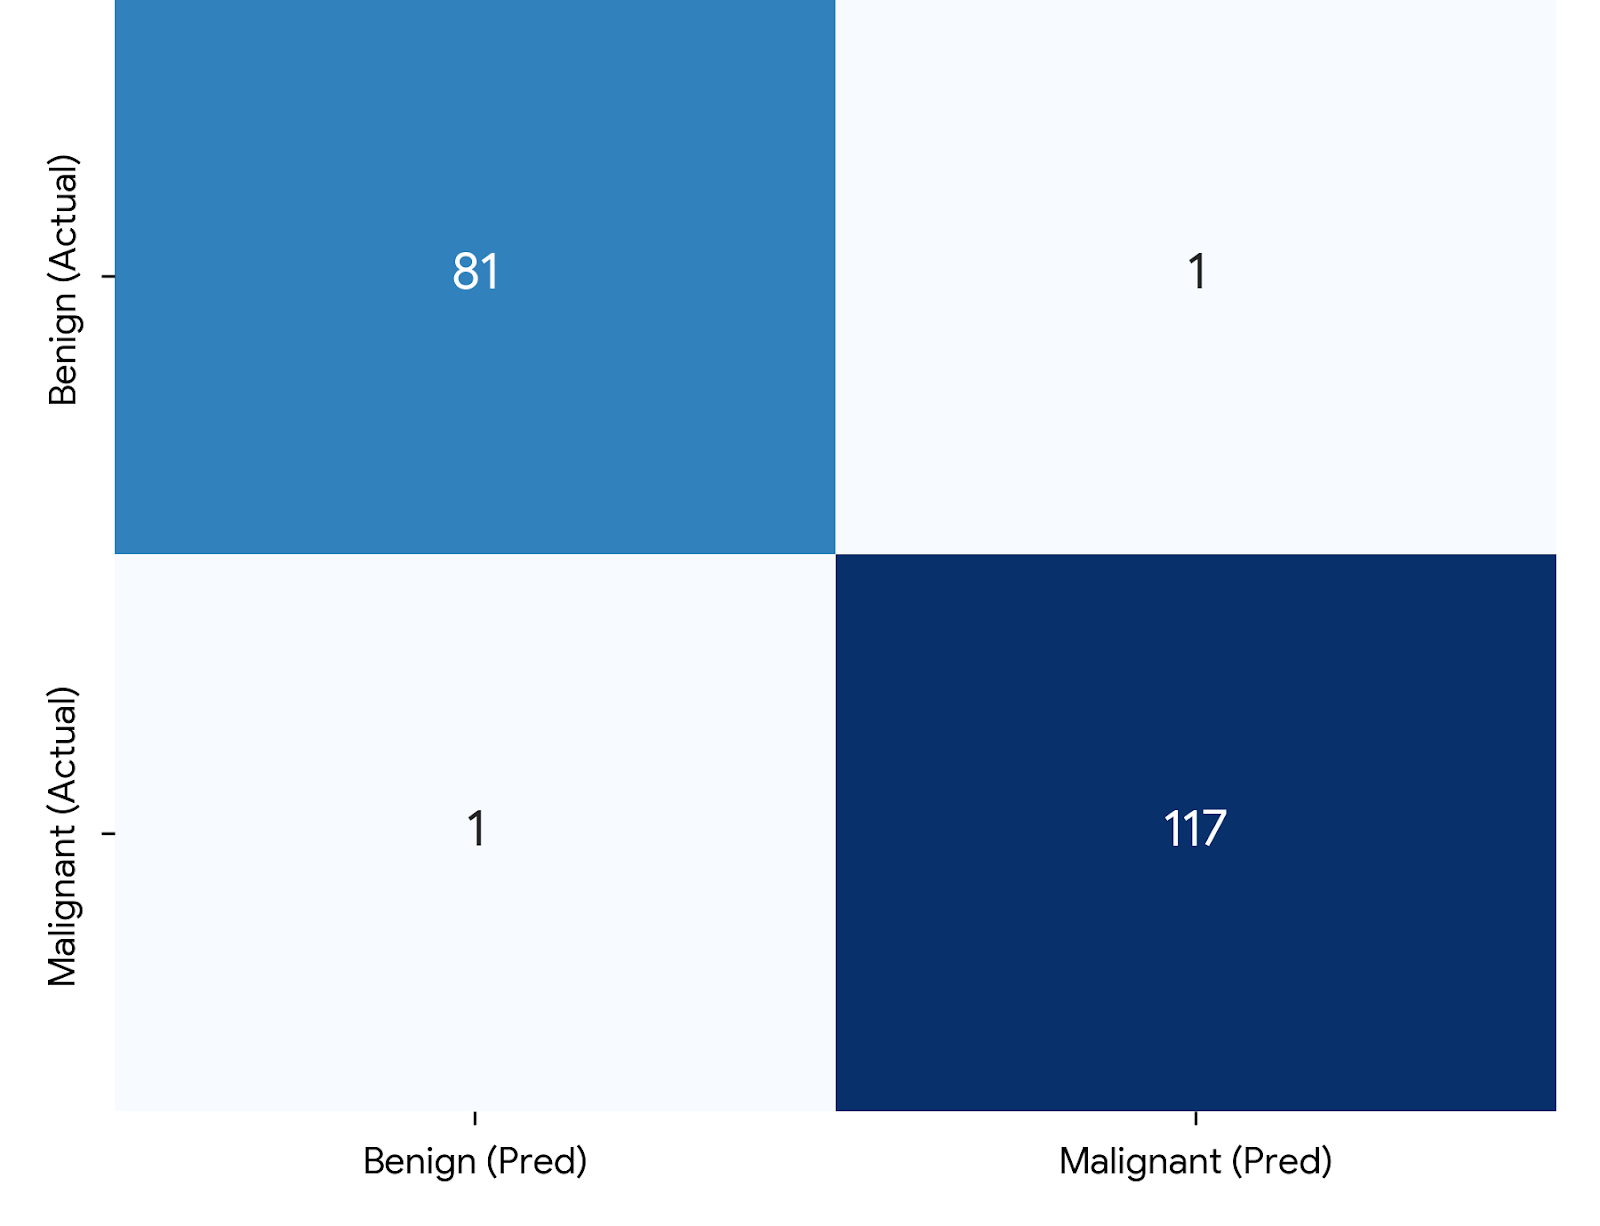
\includegraphics[width=0.75\linewidth]{figures/fig4_confusion_matrix.png}
\caption{Confusion matrix heatmap: ground truth vs. AI prediction.}
\label{fig:confusion}
\end{figure}

\FloatBarrier
\section{Discussion}
The results paint a consistent picture: benign and malignant tumors in this dataset are separated not by a single dominant feature, but by a coordinated shift across all six measured variables. This is most clearly visualized in the kernel density estimation of tumor size against mitotic count (Figure \ref{fig:kde}), where benign and malignant cases occupy almost entirely disjoint density regions along a shared diagonal axis, and in Figure \ref{fig:vascmito}, which shows vascularity rising in lockstep with mitotic count. This coordinated structure is clinically reassuring, since it means a diagnosis is not resting on a single fragile measurement; even if one feature is noisy or mismeasured for a given patient, the remaining five still point in the same direction.

\begin{figure}[h]
\centering
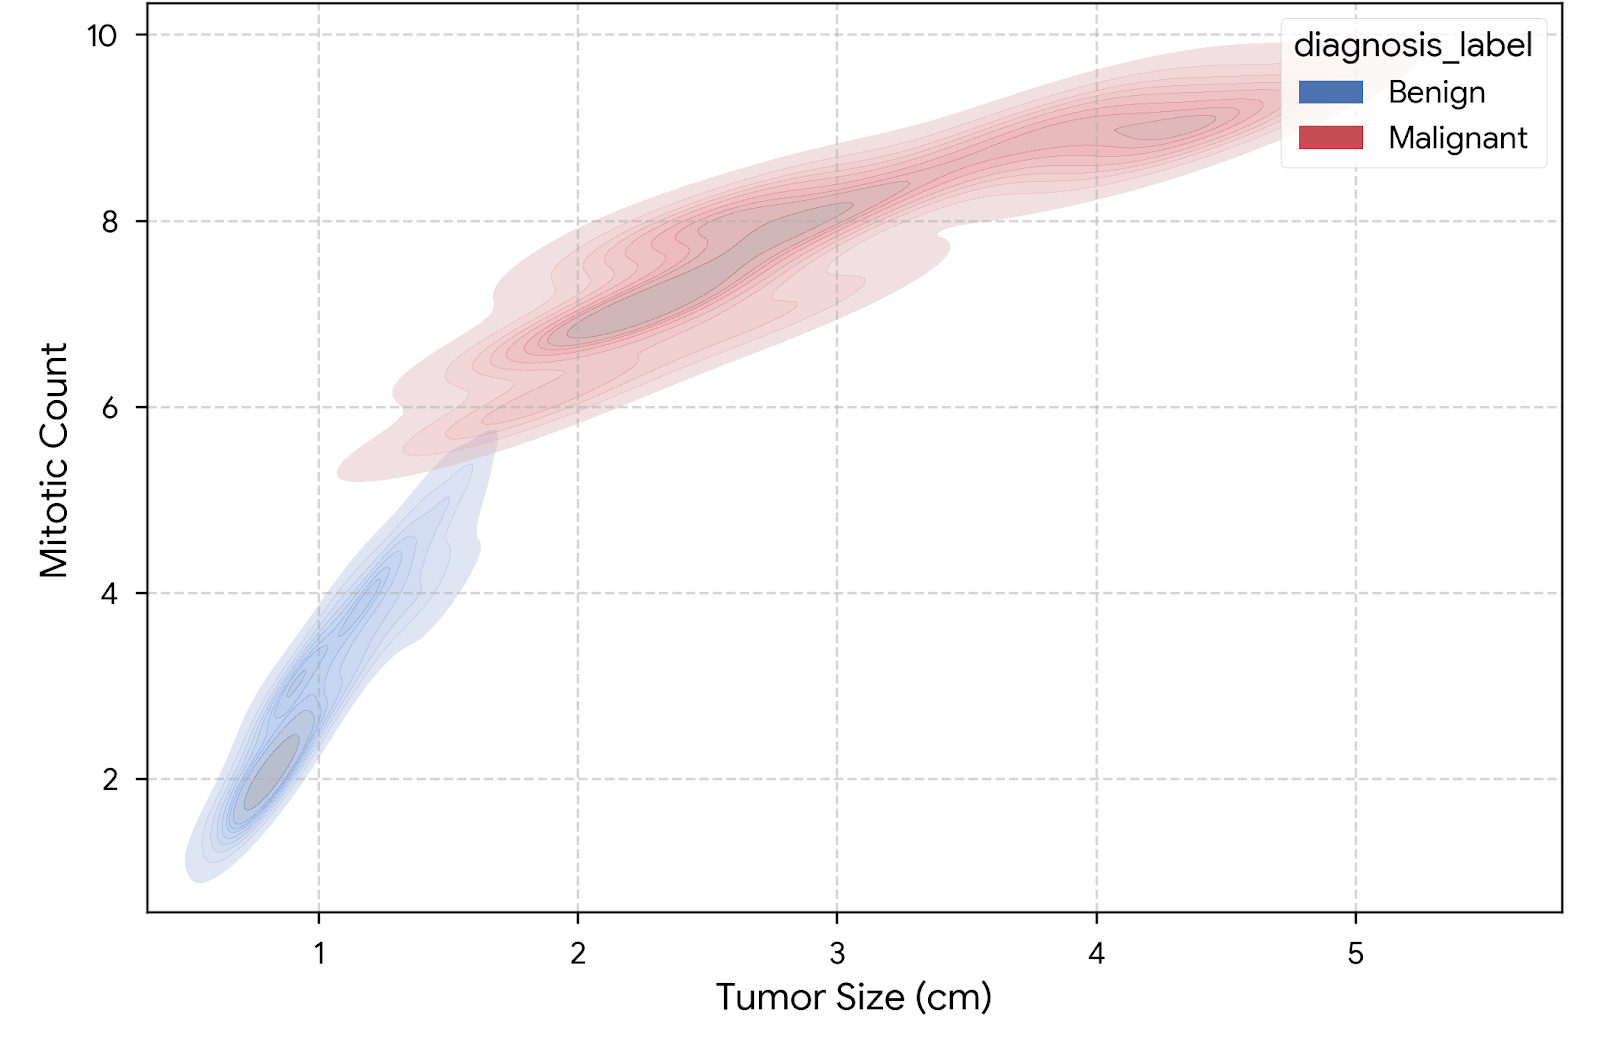
\includegraphics[width=0.75\linewidth]{figures/fig9_kde.png}
\caption{Kernel density estimation of tumor size vs. mitotic count.}
\label{fig:kde}
\end{figure}

\begin{figure}[h]
\centering
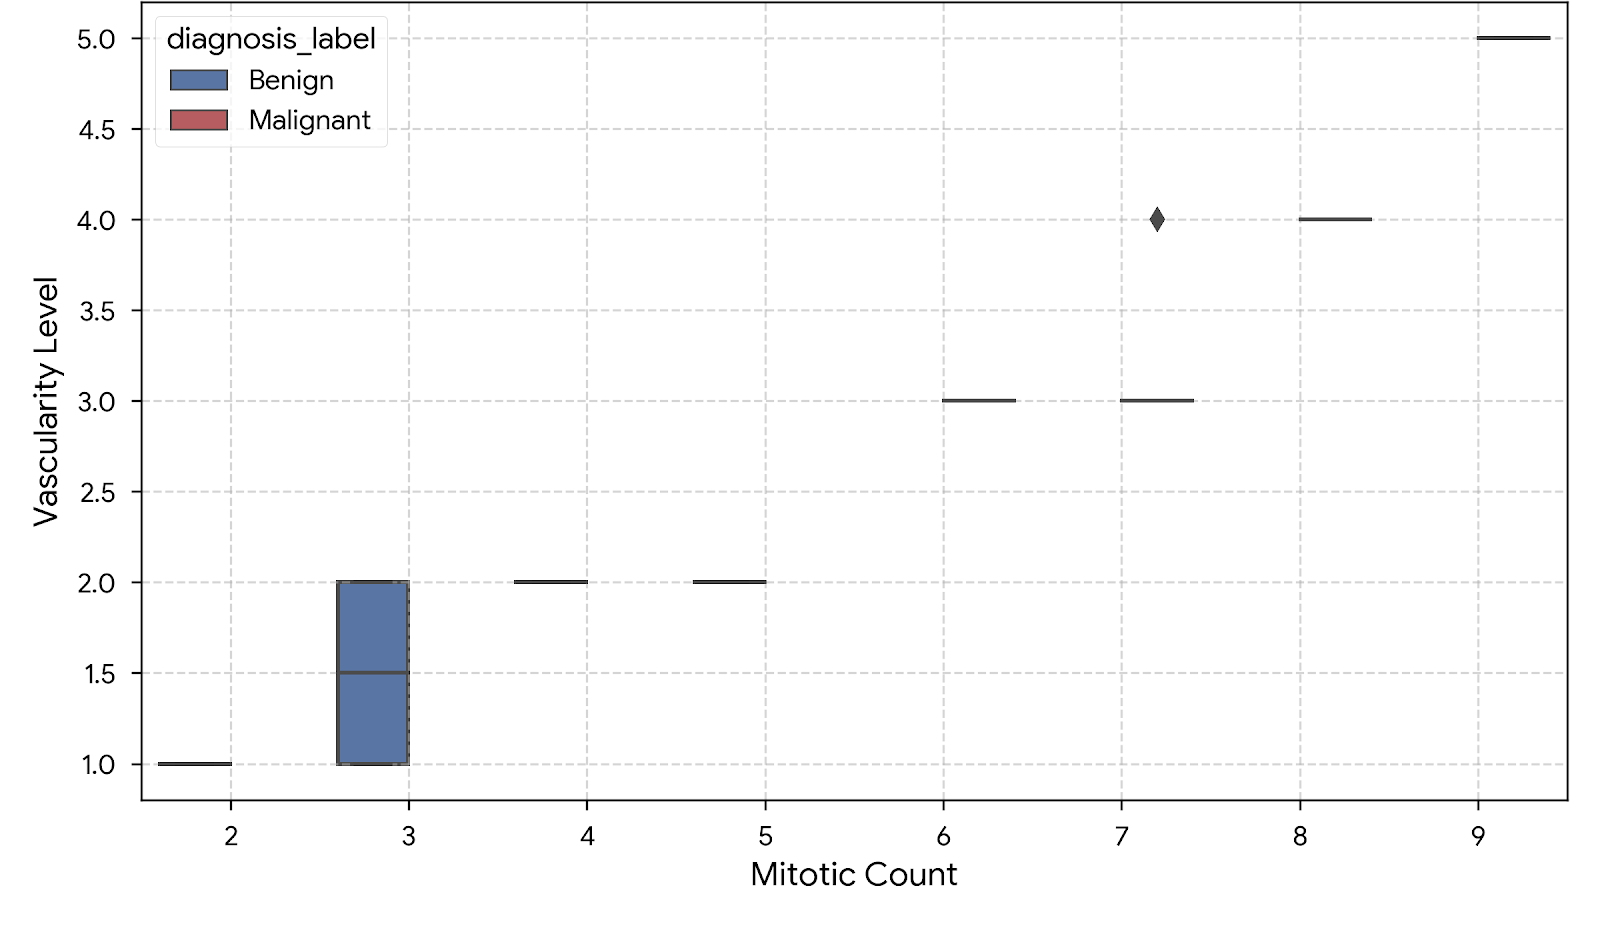
\includegraphics[width=0.75\linewidth]{figures/fig7_vascularity_mitotic.png}
\caption{Vascularity levels across mitotic counts by diagnosis.}
\label{fig:vascmito}
\end{figure}

\FloatBarrier
The AI model's 99.0\% accuracy and AUC of 1.000 are strong results, but they should be interpreted cautiously rather than as evidence the problem is fully solved. A dataset of 200 patients, however cleanly separated, is small relative to the population diversity seen in real clinical settings, and the near-perfect separability observed here may partly reflect how the six features were engineered or curated rather than the true difficulty of borderline cases in practice. Real-world tumors frequently sit closer to the diagnostic boundary than the well-separated distributions shown in Figures \ref{fig:age} and \ref{fig:ecdf}, and a classifier trained on such clean data risks overconfidence when it encounters genuinely ambiguous specimens.

Two limitations stand out. First, the dataset does not report imaging modality, biopsy technique, or inter-pathologist agreement, all of which affect real diagnostic uncertainty and are not captured by these six numeric features alone. Second, the two misclassifications, while few, both occurred near the natural boundary regions in age, size, and irregularity, reinforcing that model errors concentrate exactly where clinical uncertainty is already highest -- precisely the cases where a false negative would be most costly.

Future work should validate this feature set on a larger, multi-institution cohort, incorporate calibrated probability outputs rather than binary predictions so that borderline cases can be flagged for human review, and test robustness against measurement noise in individual features such as mitotic count, which can vary between observers. Combining the interpretable feature-based approach studied here with image-derived deep learning features, as explored in \cite{esteva2017dermatologist} and \cite{mckinney2020international}, may offer the best balance of accuracy and clinical trust.

\section{Conclusion}
This study analyzed 200 patient records to characterize how six histopathological features distinguish benign from malignant tumors and to evaluate an AI-assisted classifier against ground truth. Malignant cases showed consistently higher age, tumor size, cell irregularity, mitotic count, vascularity, and texture scores, with mitotic count and cell irregularity emerging as the strongest individual correlates of diagnosis. The AI model achieved 99.0\% accuracy with only two misclassifications, both occurring in ambiguous mid-range feature regions. These findings support quantitative, feature-based screening as a promising complement to pathologist review, while underscoring the need for larger and more heterogeneous datasets before such tools are deployed clinically.

\bibliographystyle{plain}
\bibliography{cancer_references}

\vspace{6pt}
\noindent\rule{\linewidth}{0.4pt}
\footnotesize\textit{Note: This research was conducted using publicly available academic resources, multiple AI-assisted research tools (including Claude, Gemini, Qwen, Elicit, and ChatGPT), and the author's own analytical reasoning and technical expertise. Every effort has been made to ensure academic integrity throughout the research process. This work is not intended to infringe upon the intellectual property rights, integrity, or other legal rights of any individual, institution, or organization.}

\end{document}